\subsection{LED controller}
The LED controller board is made to control all the lights. Naiad will have two sets of light containing two regular and one ir-headlight. One pointing forward and one downward. It will also have two RGB LEDs on each wing to make it easier to understand decisions made by Naiad. The LED card has two power supplies. One from the PSU powering the LEDs and one from the CAN-card powering the logical circuit. The RGB LEDs on the wings is controlled by a CAN-card through a SPI interface. To activate an LED 16 bits needs to be sent. The headlights is controlled by a PWM signal. One PWM signal for the headlights facing forward and one for the headlights facing downwards. The duty cycle of the PWM signal determines the brightness of the headlights. The experimental LED-controller board can be seen in fig. \ref{LedImgText}.

\begin{figure}[!ht]
	\begin{center}
		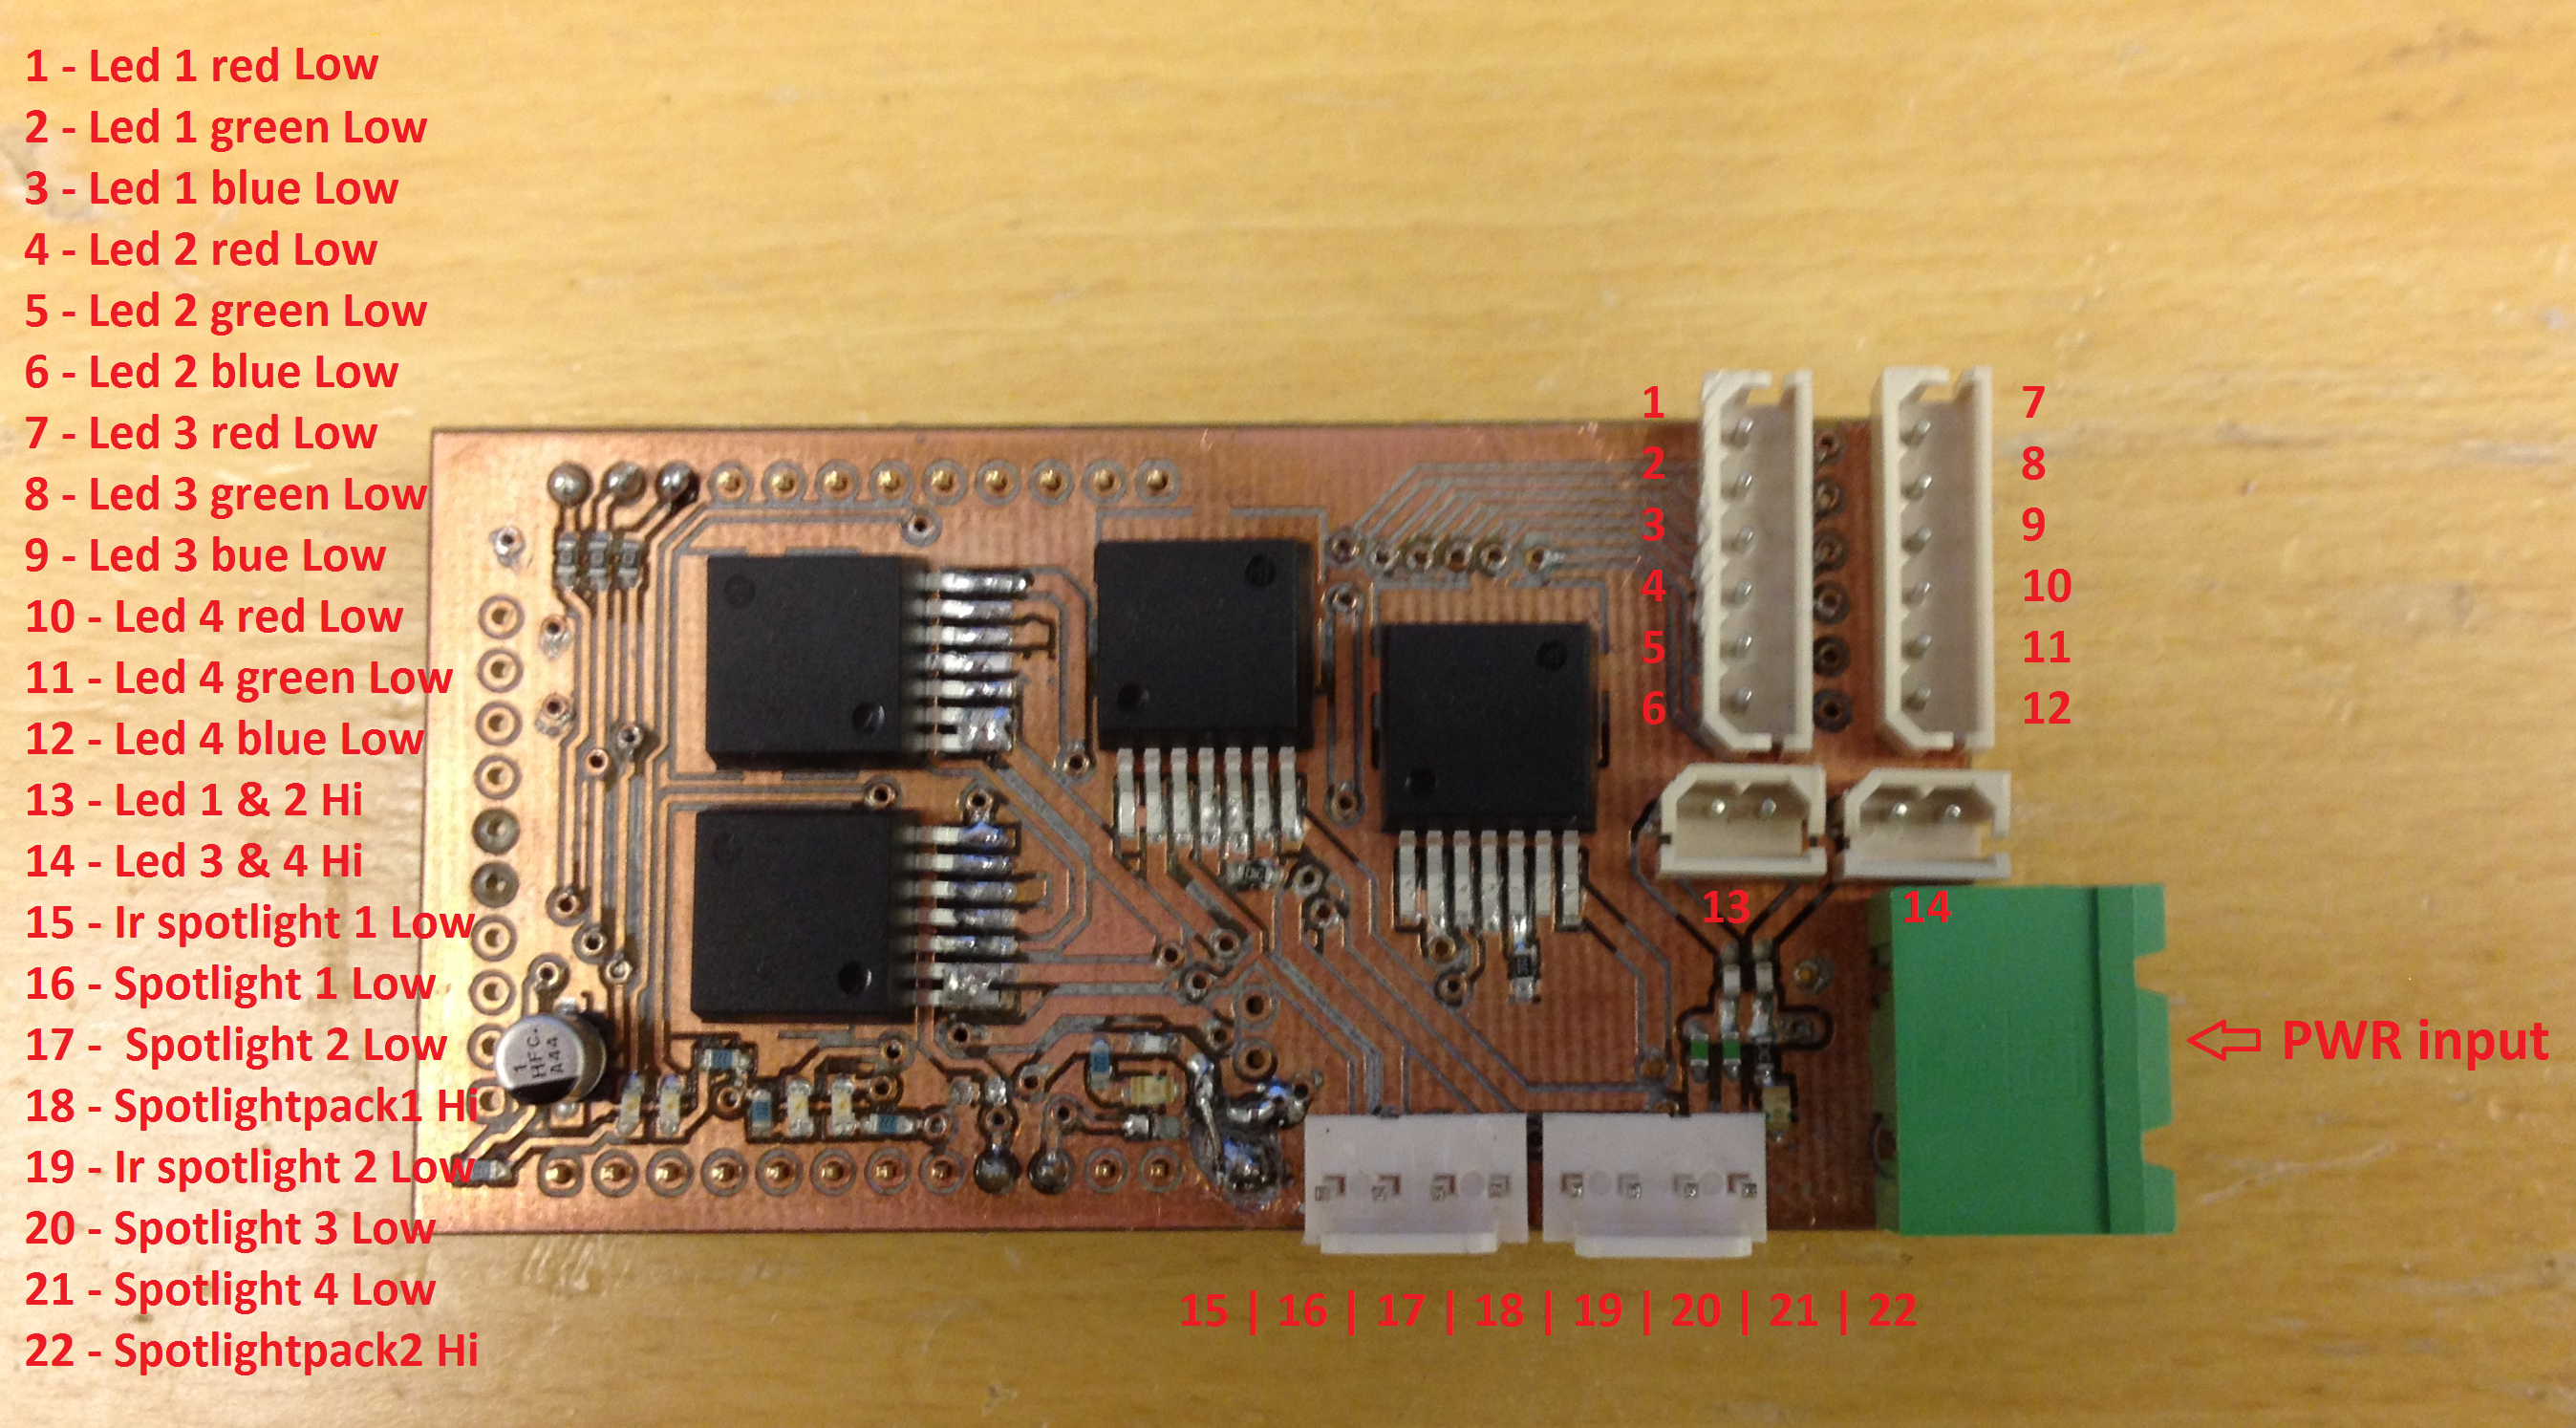
\includegraphics[width=80mm]{./Images/Electronics/LedImgtext.png}
		\caption{Picture of the experimental LED controller board}
		\label{LedImgText}
	\end{center}
\end{figure}

	
